% !TeX root = ../main.tex

\chapter{电学性质的定义、举例与相关讨论}

\section{能带理论}

固体的电学性质(即电子学性质)是从能带理论出发讨论的:在固体中,大量的分子(或原子)堆积在一起,复杂而繁多的分子轨道(或原子轨道)相互作用会形成不同的能态。能态的完整光谱带称为能带。

在一个能带中,能态不是均匀分布的。状态函数$n(E)$定义为在$E$和$E+\delta$之间的$E$的能态个数,态密度图($E-N$图)可以很好地显示能带结构。

根据能带分布和电子填充的不同,能量有不同的性质和名称:充满电子的能带称为满带,能级最高的满带称为价带;没有电子的能带称为空带,能级最低的空带称为导带(注:不同文献对导带的定义不同,也有文献称部分充满电子的能带为导带);仅部分充满电子的能带称为部分充满能带;能级之间不能被电子填充的区域称为禁带(又称禁带,记作$Eg$)。 $0K$时,电子从最低能级开始一一填满,电子占据的最高能级称为费米能级。

绝缘体只有满带和空带(导带与价带分开),$Eg$很宽($\geq 5eV$)。在一般电场条件下,价带的电子很难激发到导电状态,电子运动状态不能改变,所以不能导电。其状态密度图如下图(c)所示;半导体也只有满带和空带(导带和价带是分开的),但Eg很窄($\leq 3eV$),在一定的电场激发下可以导电。其状态密度如下图(d)所示;导体能带的结构分为两种:一种是自身就存在的部分填充的能带(直接由分子轨道或原子轨道相互作用形成而非两能带作用形成),另一种部分填充的能带由其空带、满带重叠形成,如下图(a)(b)所示。前一种导体典型的有金属钠和金属铜,后一种导体典型的有金属钙和金属锌。

(注:超导体理论将在后续的内容中单独叙述。)
\begin{figure}
    \centering
    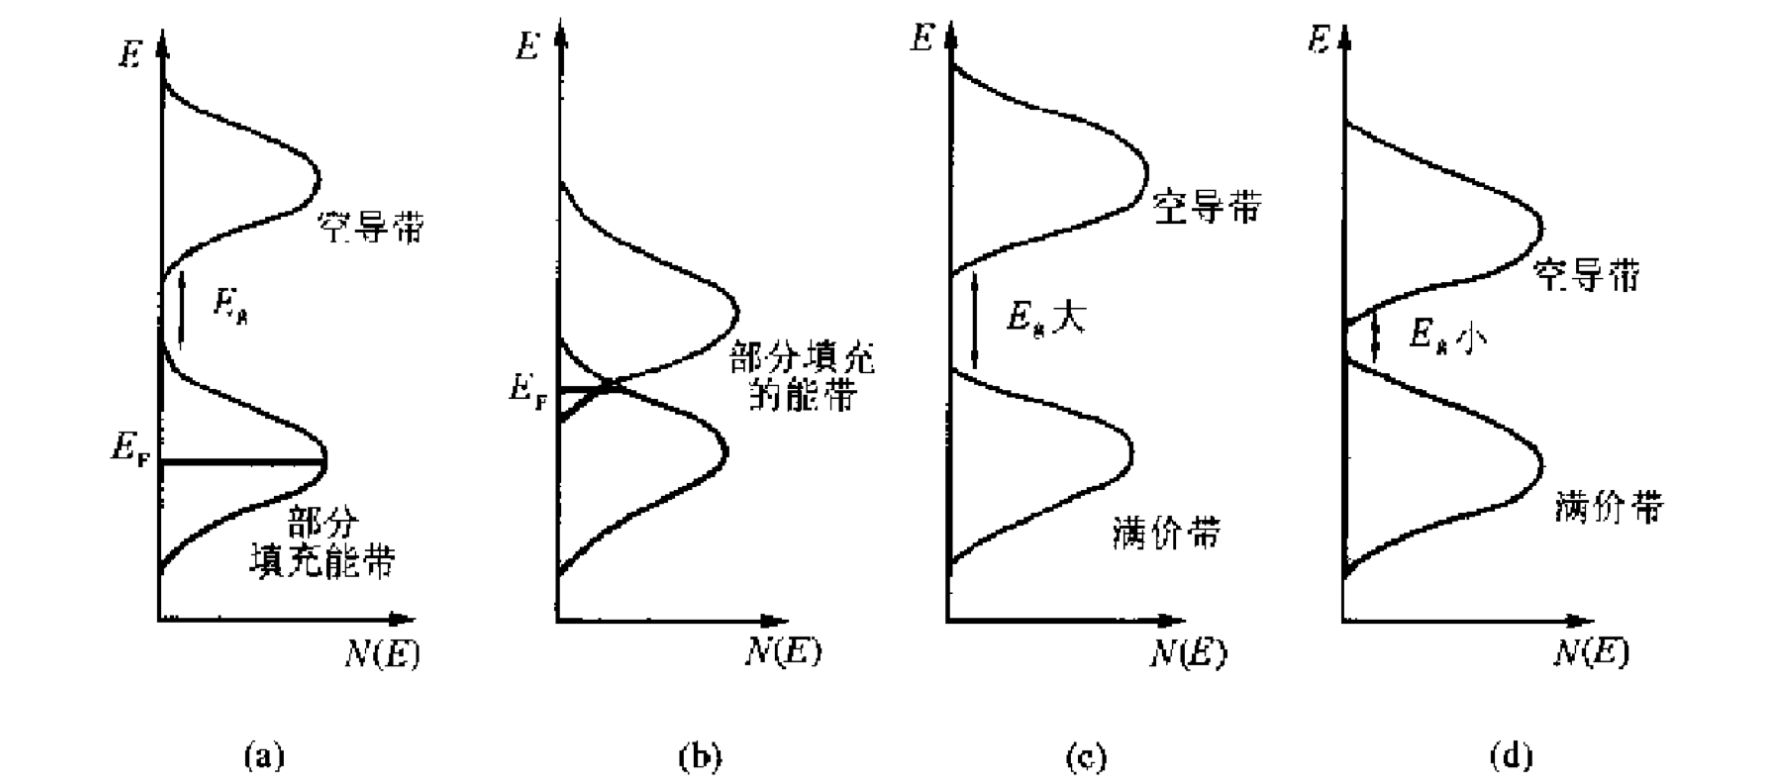
\includegraphics[scale=0.3]{img/能带.png}
    \caption{能带图像}
\end{figure}

\section{能带的直观表示方法}

叙述一下能带的直观表示方式,主要有两种:能带结构图和态密度图。态密度图的定义和举例前已叙述,实际应用中也常见态密度图的横纵坐标与前述交换;根据态密度图可以分析能隙特性。

而能带结构图纵坐标仍为能量,横坐标则为根据对称性选出的点;由于晶体的周期性,薛定谔方程的解也具有周期性,从而能带结构图可以研究整个体系各个点的能量。通过能带结构图,可以判断直接带隙或间接带隙,观察带隙、价带顶与
导带底能量。

\begin{figure}
    \centering
    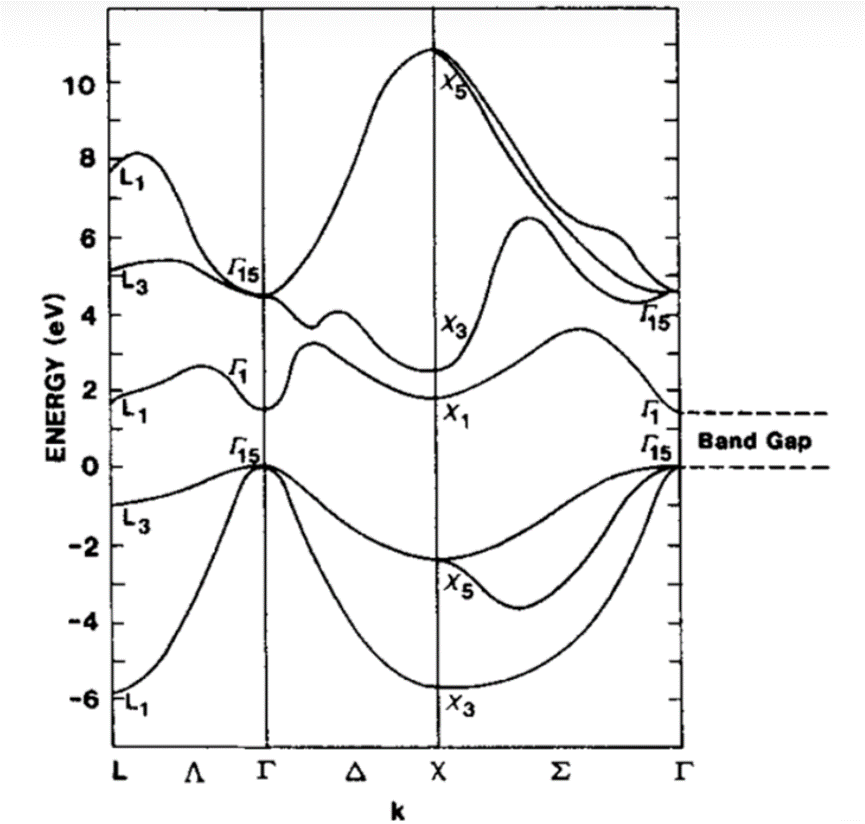
\includegraphics[scale=0.8]{img/能带结构图.png}
    \caption{能带结构图}
\end{figure}